\hypertarget{rectangle_8cpp}{
\subsection{/home/luiggi/Documents/Research/Meshless\_\-RBF/NEW/RBFSoft/examples/01TestKnots/rectangle.cpp File Reference}
\label{rectangle_8cpp}\index{/home/luiggi/Documents/Research/Meshless\_\-RBF/NEW/RBFSoft/examples/01TestKnots/rectangle.cpp@{/home/luiggi/Documents/Research/Meshless\_\-RBF/NEW/RBFSoft/examples/01TestKnots/rectangle.cpp}}
}
Testing the \hyperlink{classRectangleKnots}{RectangleKnots} class.  




\subsubsection{Detailed Description}
Testing the \hyperlink{classRectangleKnots}{RectangleKnots} class. 

In this example some features of the class \hyperlink{classRectangleKnots}{RectangleKnots} are tested. Particularly the function \hyperlink{classKnots_dd136cbe2ce6474885aab4829576472b}{Knots::findNeighbors()} is used to find the neighborhood of a target point. \begin{Desc}
\item[Input ]The {\tt inputRectangle} file contains the input data required for this program: {\tt hx} length in x-axis; {\tt hy} length in y-axis; {\tt Nx} number of points in x-axis; {\tt Ny} number of points in y-axis; {\tt rtype} knots distribution, (0 unif, 1 rand, 2 rand unif); {\tt ep} degree of randomness. {\tt layer} 0 no ghost points, 1 one layer of ghost points \end{Desc}
\begin{Desc}
\item[Output]{\tt xyzRect.dat} coordinates of random points; {\tt tarRect.dat} the target point; {\tt neiRect.dat} list of neighbors of the target. \end{Desc}
\begin{Desc}
\item[Post-procesing]You can plot the results using the next command in gnuplot: 

\footnotesize\begin{verbatim}
    % gnuplot> p "neiRect.dat" w lp, "xyzRect.dat" w p, "tarRect.dat" w p \end{verbatim}
\normalsize
 \end{Desc}
 \begin{Image}
\begin{center}
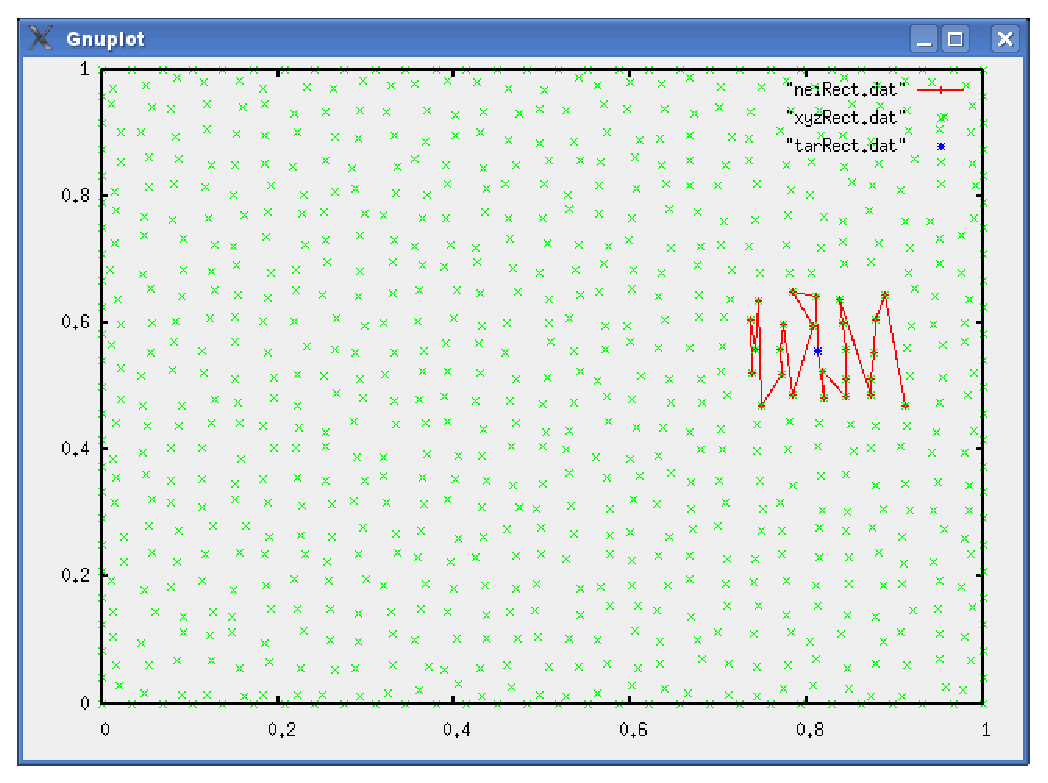
\includegraphics[width=5cm]{rectest}\caption{Knots, target and neighborhood.}
\end{center}
\end{Image}


\begin{Desc}
\item[Author:]Luis M. de la Cruz \mbox{[} Thu Sep 6 14:35:41 BST 2007 \mbox{]} \end{Desc}


Definition in file \hyperlink{rectangle_8cpp-source}{rectangle.cpp}.